%%%
% set up document type
%%%
\documentclass[12pt]{article}

%%%
% declare all packages
%%%
\usepackage[left=25mm, top=20mm, right=25mm, bottom=30mm,nohead,nofoot]{geometry} 

\usepackage[T2A]{fontenc}
\usepackage[utf8]{inputenc}
\usepackage[english, russian]{babel}

\usepackage{graphics, graphicx}

\usepackage{url}
\usepackage{hyperref}

\usepackage{amssymb,latexsym} 
\usepackage{MnSymbol}
\usepackage{mathrsfs}

\usepackage[nottoc,numbib]{tocbibind}
\usepackage{float}
\usepackage{listings}
\usepackage{multirow}
\usepackage{hhline}

\usepackage{color,colortbl}

%%%
% document settings
%%%
\setcounter{tocdepth}{4}
\graphicspath{ {./pic/} }

\renewcommand{\listoffigures}{\begingroup  % add number to list of graphics
\tocsection
\tocfile{\listfigurename}{lof}
\endgroup}
\renewcommand{\listoftables}{\begingroup  % add number to list of tables
\tocsection
\tocfile{\listtablename}{lot}
\endgroup}

%******************************************************************
%******************************************************************
\begin{document}

\begin{titlepage}
	\center
		Санкт-Петербургский Политехнический 
		университет \\ Петра Великого\\
		Институт прикладной математики и механики
		\\ \textbf{Кафедра «Прикладная математика»}

	\vfill ~
	\textbf{
		\\ \large КУРСОВАЯ РАБОТА
	}
	\\	на тему 
	\\ "Геометрические моды колебаний плазмы"
	\\ по дисциплине
	\\ "Математическая статистика"

	\vfill ~

	Выполнил студент гр. \textbf{33631/1} \\
	\textbf{Лансков.Н.В.} \\ 

\vfill

{\large}	Санкт-Петербург
\\ 2019
\end{titlepage}

%%%
% Table of conetnts 
%%%

\tableofcontents 
\newpage
\listoffigures
\newpage
% \listoftables
% \newpage

%%%
% Text
%%%
\section{Описание}

\subsection{Исследование временной эволюции светимости плазмы во время разряда.}
\begin{center}

\begin{figure}[H]
\caption{Графики светимости "северной" и "южной" части плазмы в устойчивой фазе в течение 40 мс}
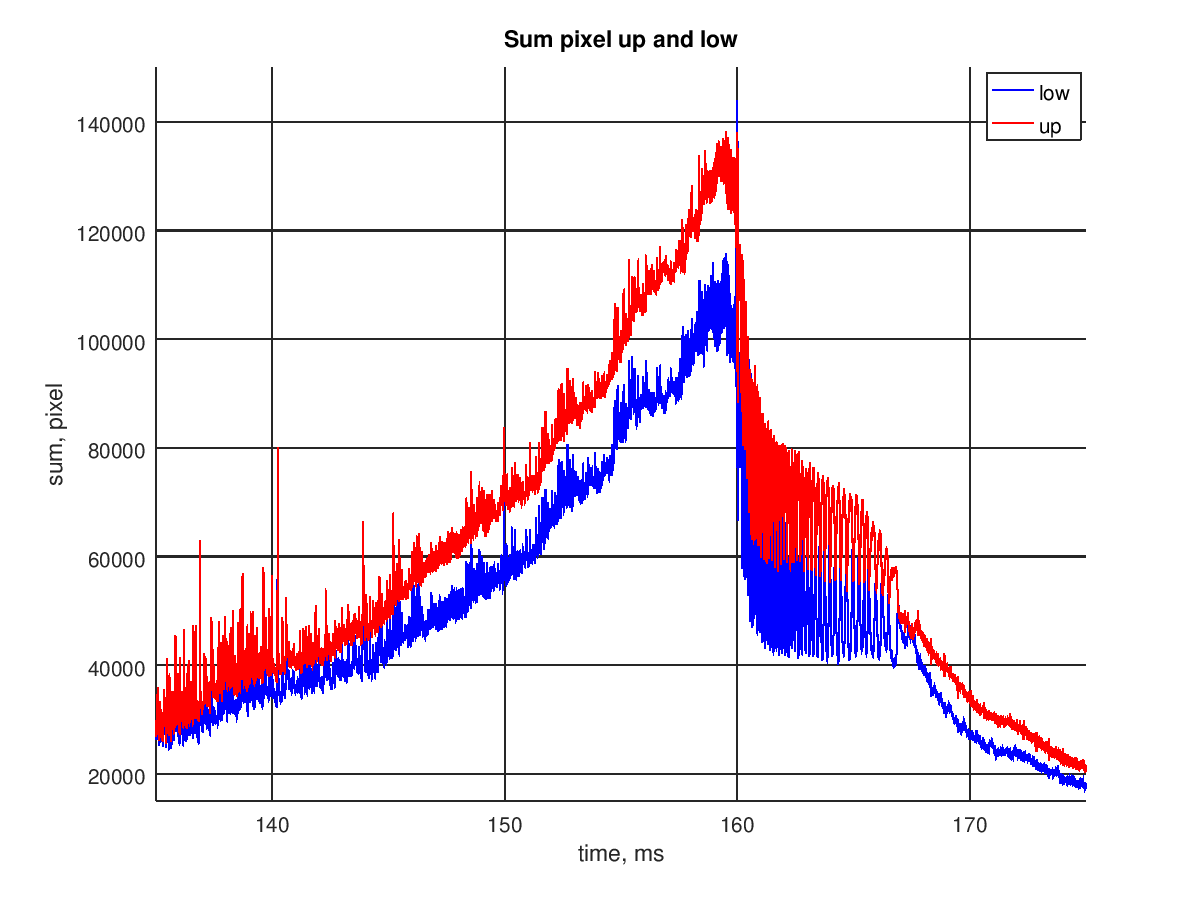
\includegraphics[scale = 0.8]{plot1.png} 
\end{figure}

\begin{figure}[H]
\caption{Графики светимости "северной" и "южной" части плазмы в устойчивой фазе в течение 3 мс}
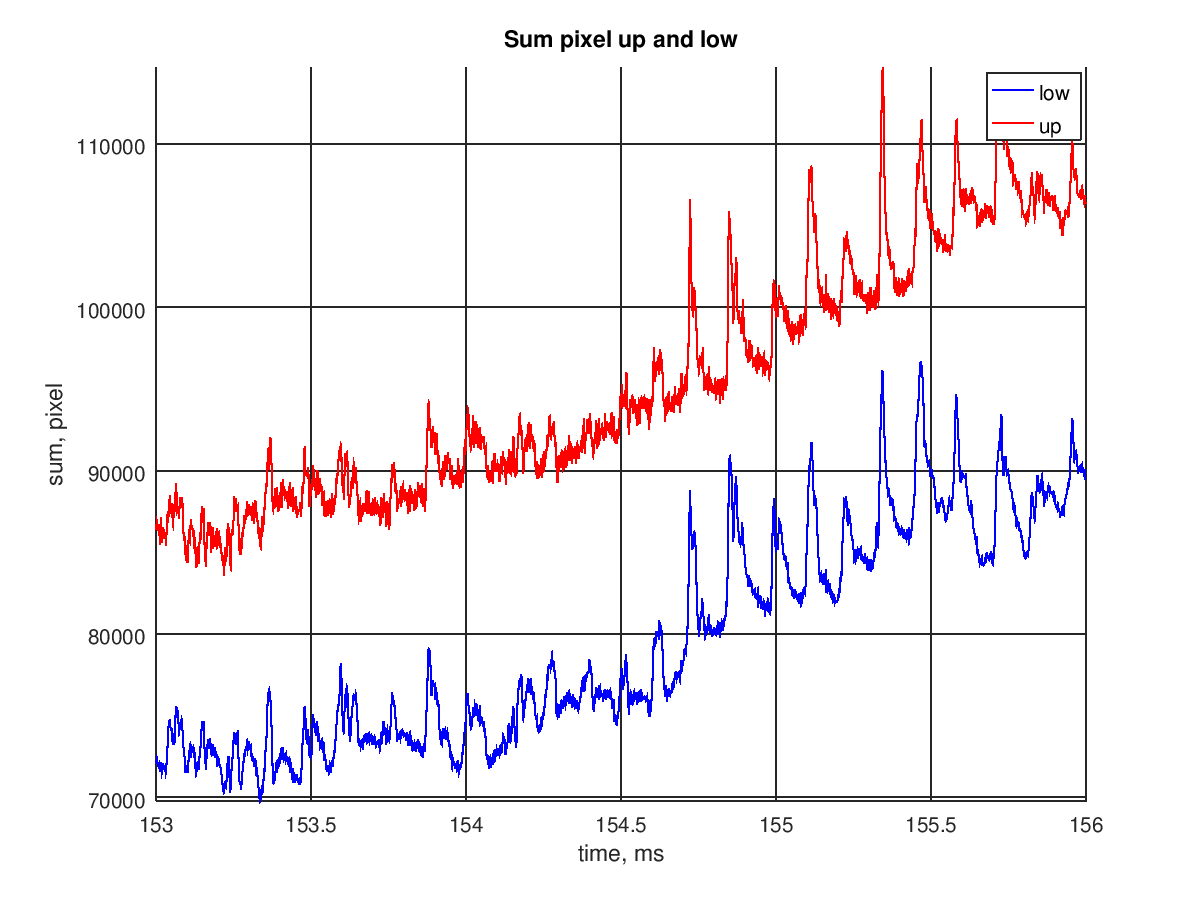
\includegraphics[scale = 0.8]{plot2.png} 
\end{figure}

\end{center}

\section{Постановка задачи}

\subsection{Подготовка данных}
\begin{enumerate}
\item Считать данные светимости.
\item Сопоставить индексы с временной шкалой.
\item Выделить области светимости выше и ниже экватора.
\end{enumerate}

\subsection{Рассчёты}
\begin{enumerate}
\item Ввести временное окно 1 мс.
\item Рассчитать коэффициент корреляции R между светимостями областей выше и ниже экватора.
\item Запомнить сдвиг по времени, доставляющий максимум этой функции.
\item По данным построить гистограмму сдвигов по времени.
\end{enumerate}

\section{Теория}
Пусть по выборке значений двумерной $ \{x_{i}, y_{i}\}^{n}_{1} $ с.в. $ (X, Y) $ требуется оценить коэффициент корреляции $ \rho_{XY} = \dfrac{cov(X, Y)}{\sqrt{DX DY}}  $. Естественной оценкой для $ \rho_{XY} $ служит его статистический аналог в виде выборочного коэффициента корреляции, предложенного К. Пирсоном, -

\begin{equation}
r = r_{XY} = \dfrac{\dfrac{1}{n}\Sigma{(x_{i} - \overline{x})(y_{i} - \overline{y})}}{\sqrt{\dfrac{1}{n^{2}} \Sigma(x_{i} - \overline{x})^{2} \Sigma(y_{i} - \overline{y})^{2}}} = \dfrac{K_{XY}}{s_{X}s_{Y}},  \label{eqn:corr}
\end{equation}

где $K_{XY}, s_{X}^{2}, s_{Y}^{2}$ - выборочные ковариация и дисперсии с.в. $X$ и $Y$.
Из теории вероятностей известно, что коэффициент корреляции является мерой линейной стохастической зависимости между случайными величинами. Соответственно, выборочный коэффициент корреляции как его статистический аналог наследует и другие свойства генерального коэффициента корреляции:

\begin{enumerate}
\item $-1 \geq r \leq +1;$
\item если $y_{i} = a_{i}x_{i} + b_{i}, i = \overline{1, n}, a \neq 0, $ то $r = + 1$ при $a\leq 0$ и $r = - 1$ при $a\geq 0$
\end{enumerate}

Чем сильнее линейная связь между переменными $X$ и $Y$, тем ближе |r| к 1; чем ближе r к нулю, тем слабее исследуемая линейная связь.
Отметим, что близость к нулю выборочного коэффициента корреляции указывает только на отсутствие линейной связи между переменнымиж вполне возможно, что при этом между ними имеется нелинейная связь.
Как видно из формулы (\ref{eqn:corr}), выборочный коэффициент корреляции является симметричной функцией переменных $X$ и $Y$, и только количественно выражает связь между этими переменными.\cite{max}
\section{Реализация}
Выполнено средствами \textbf{MATLAB(GNU Octave)}.

\section{Результаты}

\begin{figure}[H]
\caption{Коэффициент корреляции R между светимостями областей выше и ниже экватора.}
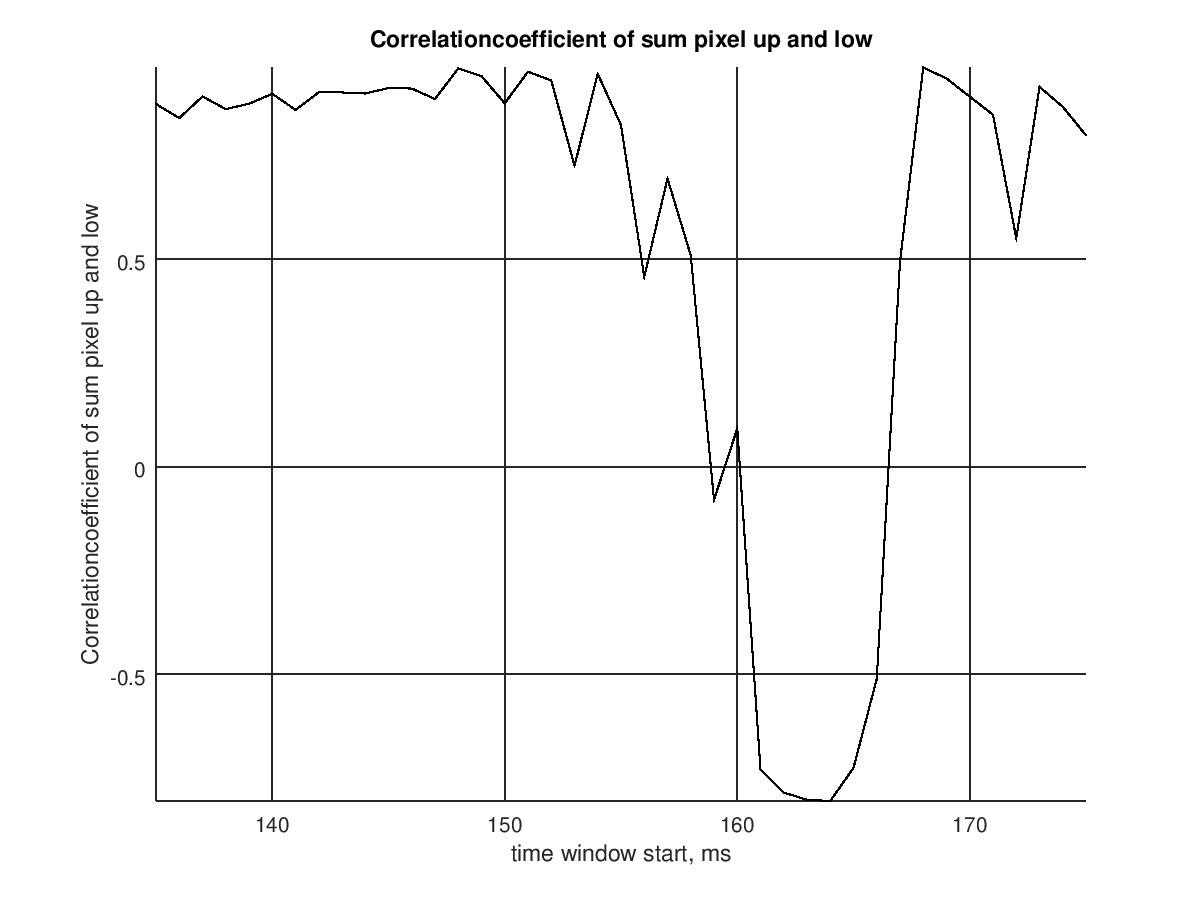
\includegraphics[scale = 0.8]{plot3.png} 
\end{figure}

Сдвиг по времени, на котором коэффициент корелляции достигает максимального значения.
$$ shift(max) = [168, 169] $$

\begin{figure}[H]
\caption{Гистограмма (коэффициент корреляции / сдвиг по времени)}
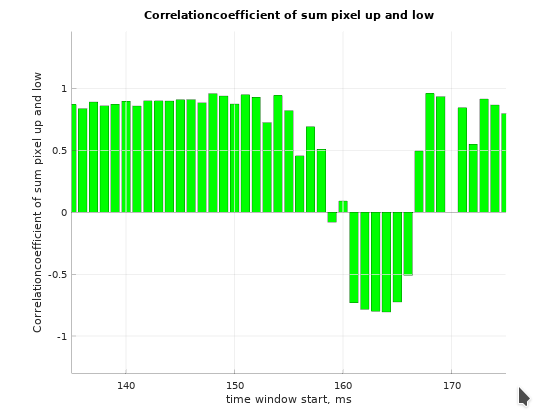
\includegraphics[scale = 1]{plot4.png} 
\end{figure}

\section{Приложения}

\textbf{Исходники:} \\
\url{https://github.com/LanskovNV/math_statistics/tree/master/course_proj}

% \newpage

%%%
% Literature
%%%
\begin{thebibliography}{}
    \bibitem{max}
    \textbf{Вероятностные разделы математики.} \\
    Учебник для бакалавров технических направлений.//Под редакцией Максимова.Ю.Д. - Спб.: "Иван Фёдоров", 2001.  
\end{thebibliography}

\end{document}

